\subsection{Reflecting on Yagis: The Magic of Two-Element Designs!}

\begin{tcolorbox}[colback=gray!10, colframe=black, title=E9D11]
Why do most two-element Yagis with normal spacing have a reflector instead of a director? 

\begin{enumerate}
    \item A: Lower SWR
    \item B: Higher receiving directivity factor
    \item C: Greater front-to-side
    \item D: \textbf{Higher gain}
\end{enumerate} \end{tcolorbox}

\subsubsection{Concepts and Explanation}

To understand why most two-element Yagi antennas utilize a reflector instead of a director, it is important to grasp some foundational concepts of antenna design and functionality. 

A Yagi-Uda antenna typically consists of a driven element (which is fed with the RF signal), and additional elements that can be either directors or reflectors, positioned in relation to the driven element. 

1. \textbf{Reflector vs. Director:} 
   - A reflector is placed behind the driven element and serves to reflect the radiated energy back towards the front, thus providing an increase in gain in the forward direction. 
   - A director is placed in front of the driven element, enhancing its directivity by focusing the signal in a specific direction. 

2. \textbf{Antenna Gain:} 
   - Gain is the measure of an antenna's ability to direct radio frequency energy in a particular direction compared to an isotropic radiator (a hypothetical antenna that radiates equally in all directions).
   - A two-element Yagi antenna with a reflector can achieve higher gain than a simple dipole or an antenna with only directors.

3. \textbf{Normal Spacing:} 
   - Normal spacing in this context typically refers to the spacing between the elements being optimal for maximum performance. For many Yagi designs, this spacing is commonly about 0.1 to 0.2 wavelengths apart.

In conclusion, the reason why most two-element Yagis often incorporate a reflector instead of adding a director is primarily due to the increase in the gain of the antenna. Adding a reflector enhances the overall radiation pattern and focuses the transmitted energy more effectively, yielding higher gain as compared to using only directors.

\subsubsection{Mathematical Consideration}

It can be insightful to calculate the gain difference theoretically. While detailed calculations would require known formulas and numerical values specific to the antenna configuration, we can summarize the gain \( G \) of a Yagi-Uda antenna in decibels (dB):

\[
G \approx 10 \log_{10} \left( \frac{P_{\text{radiated}}}{P_{\text{input}}} \right)
\]

Where \( P_{\text{radiated}} \) is the power radiated in a specific direction, and \( P_{\text{input}} \) is the input power. 

As with any practical design, further optimizations and adjustments might be necessary based on the specific application and frequency being used.

\subsubsection{Diagram Representation}

A simple diagram of a two-element Yagi antenna can be drawn using the TikZ package as follows:

\begin{center}
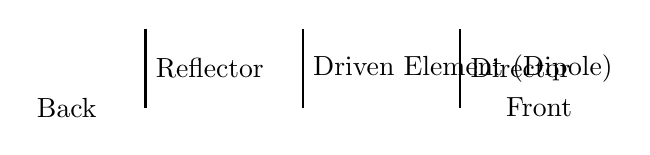
\begin{tikzpicture}
    % Draw the driven element
    \draw[thick] (0,0) -- (0,1) node[midway, right] {Driven Element (Dipole)};
    
    % Draw the reflector
    \draw[thick] (-2,0) -- (-2,1) node[midway, right] {Reflector};
    
    % Draw the director
    \draw[thick] (2,0) -- (2,1) node[midway, right] {Director};
    
    % Draw labels for indicating front and back
    \node at (-3, 0) {Back};
    \node at (3, 0) {Front};
\end{tikzpicture}
\end{center}
